\documentclass{ximera}  


%\usepackage{todonotes}
%\usepackage{mathtools} %% Required for wide table Curl and Greens
%\usepackage{cuted} %% Required for wide table Curl and Greens
\newcommand{\todo}{}

\usepackage{esint} % for \oiint
\ifxake%%https://math.meta.stackexchange.com/questions/9973/how-do-you-render-a-closed-surface-double-integral
\renewcommand{\oiint}{{\large\bigcirc}\kern-1.56em\iint}
\fi


\graphicspath{
  {./}
  {jpg}
  {ximeraTutorial/}
  {basicPhilosophy/}
  {functionsOfSeveralVariables/}
  {normalVectors/}
  {lagrangeMultipliers/}
  {vectorFields/}
  {greensTheorem/}
  {shapeOfThingsToCome/}
  {dotProducts/}
  {partialDerivativesAndTheGradientVector/}
  {../productAndQuotientRules/exercises/}
  {../motionAndPathsInSpace/exercises/}
  {../normalVectors/exercisesParametricPlots/}
  {../continuityOfFunctionsOfSeveralVariables/exercises/}
  {../partialDerivativesAndTheGradientVector/exercises/}
  {../directionalDerivativeAndChainRule/exercises/}
  {../commonCoordinates/exercisesCylindricalCoordinates/}
  {../commonCoordinates/exercisesSphericalCoordinates/}
  {../greensTheorem/exercisesCurlAndLineIntegrals/}
  {../greensTheorem/exercisesDivergenceAndLineIntegrals/}
  {../shapeOfThingsToCome/exercisesDivergenceTheorem/}
  {../greensTheorem/}
  {../shapeOfThingsToCome/}
  {../separableDifferentialEquations/exercises/}
  {vectorFields/}
}

\newcommand{\mooculus}{\textsf{\textbf{MOOC}\textnormal{\textsf{ULUS}}}}

\usepackage{tkz-euclide}\usepackage{tikz}
\usepackage{tikz-cd}
\usetikzlibrary{arrows}
\tikzset{>=stealth,commutative diagrams/.cd,
  arrow style=tikz,diagrams={>=stealth}} %% cool arrow head
\tikzset{shorten <>/.style={ shorten >=#1, shorten <=#1 } } %% allows shorter vectors

\usetikzlibrary{backgrounds} %% for boxes around graphs
\usetikzlibrary{shapes,positioning}  %% Clouds and stars
\usetikzlibrary{matrix} %% for matrix
\usepgfplotslibrary{polar} %% for polar plots
\usepgfplotslibrary{fillbetween} %% to shade area between curves in TikZ
\usetkzobj{all}
\usepackage[makeroom]{cancel} %% for strike outs
%\usepackage{mathtools} %% for pretty underbrace % Breaks Ximera
%\usepackage{multicol}
\usepackage{pgffor} %% required for integral for loops



%% http://tex.stackexchange.com/questions/66490/drawing-a-tikz-arc-specifying-the-center
%% Draws beach ball
\tikzset{pics/carc/.style args={#1:#2:#3}{code={\draw[pic actions] (#1:#3) arc(#1:#2:#3);}}}



\usepackage{array}
\setlength{\extrarowheight}{+.1cm}
\newdimen\digitwidth
\settowidth\digitwidth{9}
\def\divrule#1#2{
\noalign{\moveright#1\digitwidth
\vbox{\hrule width#2\digitwidth}}}





\newcommand{\RR}{\mathbb R}
\newcommand{\R}{\mathbb R}
\newcommand{\N}{\mathbb N}
\newcommand{\Z}{\mathbb Z}

\newcommand{\sagemath}{\textsf{SageMath}}


%\renewcommand{\d}{\,d\!}
\renewcommand{\d}{\mathop{}\!d}
\newcommand{\dd}[2][]{\frac{\d #1}{\d #2}}
\newcommand{\pp}[2][]{\frac{\partial #1}{\partial #2}}
\renewcommand{\l}{\ell}
\newcommand{\ddx}{\frac{d}{\d x}}

\newcommand{\zeroOverZero}{\ensuremath{\boldsymbol{\tfrac{0}{0}}}}
\newcommand{\inftyOverInfty}{\ensuremath{\boldsymbol{\tfrac{\infty}{\infty}}}}
\newcommand{\zeroOverInfty}{\ensuremath{\boldsymbol{\tfrac{0}{\infty}}}}
\newcommand{\zeroTimesInfty}{\ensuremath{\small\boldsymbol{0\cdot \infty}}}
\newcommand{\inftyMinusInfty}{\ensuremath{\small\boldsymbol{\infty - \infty}}}
\newcommand{\oneToInfty}{\ensuremath{\boldsymbol{1^\infty}}}
\newcommand{\zeroToZero}{\ensuremath{\boldsymbol{0^0}}}
\newcommand{\inftyToZero}{\ensuremath{\boldsymbol{\infty^0}}}



\newcommand{\numOverZero}{\ensuremath{\boldsymbol{\tfrac{\#}{0}}}}
\newcommand{\dfn}{\textbf}
%\newcommand{\unit}{\,\mathrm}
\newcommand{\unit}{\mathop{}\!\mathrm}
\newcommand{\eval}[1]{\bigg[ #1 \bigg]}
\newcommand{\seq}[1]{\left( #1 \right)}
\renewcommand{\epsilon}{\varepsilon}
\renewcommand{\phi}{\varphi}


\renewcommand{\iff}{\Leftrightarrow}

\DeclareMathOperator{\arccot}{arccot}
\DeclareMathOperator{\arcsec}{arcsec}
\DeclareMathOperator{\arccsc}{arccsc}
\DeclareMathOperator{\si}{Si}
\DeclareMathOperator{\scal}{scal}
\DeclareMathOperator{\sign}{sign}


%% \newcommand{\tightoverset}[2]{% for arrow vec
%%   \mathop{#2}\limits^{\vbox to -.5ex{\kern-0.75ex\hbox{$#1$}\vss}}}
\newcommand{\arrowvec}[1]{{\overset{\rightharpoonup}{#1}}}
%\renewcommand{\vec}[1]{\arrowvec{\mathbf{#1}}}
\renewcommand{\vec}[1]{{\overset{\boldsymbol{\rightharpoonup}}{\mathbf{#1}}}\hspace{0in}}

\newcommand{\point}[1]{\left(#1\right)} %this allows \vector{ to be changed to \vector{ with a quick find and replace
\newcommand{\pt}[1]{\mathbf{#1}} %this allows \vec{ to be changed to \vec{ with a quick find and replace
\newcommand{\Lim}[2]{\lim_{\point{#1} \to \point{#2}}} %Bart, I changed this to point since I want to use it.  It runs through both of the exercise and exerciseE files in limits section, which is why it was in each document to start with.

\DeclareMathOperator{\proj}{\mathbf{proj}}
\newcommand{\veci}{{\boldsymbol{\hat{\imath}}}}
\newcommand{\vecj}{{\boldsymbol{\hat{\jmath}}}}
\newcommand{\veck}{{\boldsymbol{\hat{k}}}}
\newcommand{\vecl}{\vec{\boldsymbol{\l}}}
\newcommand{\uvec}[1]{\mathbf{\hat{#1}}}
\newcommand{\utan}{\mathbf{\hat{t}}}
\newcommand{\unormal}{\mathbf{\hat{n}}}
\newcommand{\ubinormal}{\mathbf{\hat{b}}}

\newcommand{\dotp}{\bullet}
\newcommand{\cross}{\boldsymbol\times}
\newcommand{\grad}{\boldsymbol\nabla}
\newcommand{\divergence}{\grad\dotp}
\newcommand{\curl}{\grad\cross}
%\DeclareMathOperator{\divergence}{divergence}
%\DeclareMathOperator{\curl}[1]{\grad\cross #1}
\newcommand{\lto}{\mathop{\longrightarrow\,}\limits}

\renewcommand{\bar}{\overline}

\colorlet{textColor}{black}
\colorlet{background}{white}
\colorlet{penColor}{blue!50!black} % Color of a curve in a plot
\colorlet{penColor2}{red!50!black}% Color of a curve in a plot
\colorlet{penColor3}{red!50!blue} % Color of a curve in a plot
\colorlet{penColor4}{green!50!black} % Color of a curve in a plot
\colorlet{penColor5}{orange!80!black} % Color of a curve in a plot
\colorlet{penColor6}{yellow!70!black} % Color of a curve in a plot
\colorlet{fill1}{penColor!20} % Color of fill in a plot
\colorlet{fill2}{penColor2!20} % Color of fill in a plot
\colorlet{fillp}{fill1} % Color of positive area
\colorlet{filln}{penColor2!20} % Color of negative area
\colorlet{fill3}{penColor3!20} % Fill
\colorlet{fill4}{penColor4!20} % Fill
\colorlet{fill5}{penColor5!20} % Fill
\colorlet{gridColor}{gray!50} % Color of grid in a plot

\newcommand{\surfaceColor}{violet}
\newcommand{\surfaceColorTwo}{redyellow}
\newcommand{\sliceColor}{greenyellow}




\pgfmathdeclarefunction{gauss}{2}{% gives gaussian
  \pgfmathparse{1/(#2*sqrt(2*pi))*exp(-((x-#1)^2)/(2*#2^2))}%
}


%%%%%%%%%%%%%
%% Vectors
%%%%%%%%%%%%%

%% Simple horiz vectors
\renewcommand{\vector}[1]{\left\langle #1\right\rangle}


%% %% Complex Horiz Vectors with angle brackets
%% \makeatletter
%% \renewcommand{\vector}[2][ , ]{\left\langle%
%%   \def\nextitem{\def\nextitem{#1}}%
%%   \@for \el:=#2\do{\nextitem\el}\right\rangle%
%% }
%% \makeatother

%% %% Vertical Vectors
%% \def\vector#1{\begin{bmatrix}\vecListA#1,,\end{bmatrix}}
%% \def\vecListA#1,{\if,#1,\else #1\cr \expandafter \vecListA \fi}

%%%%%%%%%%%%%
%% End of vectors
%%%%%%%%%%%%%

%\newcommand{\fullwidth}{}
%\newcommand{\normalwidth}{}



%% makes a snazzy t-chart for evaluating functions
%\newenvironment{tchart}{\rowcolors{2}{}{background!90!textColor}\array}{\endarray}

%%This is to help with formatting on future title pages.
\newenvironment{sectionOutcomes}{}{}



%% Flowchart stuff
%\tikzstyle{startstop} = [rectangle, rounded corners, minimum width=3cm, minimum height=1cm,text centered, draw=black]
%\tikzstyle{question} = [rectangle, minimum width=3cm, minimum height=1cm, text centered, draw=black]
%\tikzstyle{decision} = [trapezium, trapezium left angle=70, trapezium right angle=110, minimum width=3cm, minimum height=1cm, text centered, draw=black]
%\tikzstyle{question} = [rectangle, rounded corners, minimum width=3cm, minimum height=1cm,text centered, draw=black]
%\tikzstyle{process} = [rectangle, minimum width=3cm, minimum height=1cm, text centered, draw=black]
%\tikzstyle{decision} = [trapezium, trapezium left angle=70, trapezium right angle=110, minimum width=3cm, minimum height=1cm, text centered, draw=black]




 
\title{Electrostatic fields from distributed charges} 
\author{Milica Markovic} 
\outcome{Distributed charges.}
\begin{document}  
\begin{abstract}  

\end{abstract}  
\maketitle    


\section{Electric Field due to a Charge Distribution}

\subsection{Derive Analytical Solution for the Electric field Due to a Loop of Charge }



We will first find the electric field due to a loop of charge.The loop of charge is charged with the line charge density $\rho_l$ and is in X-Y plane, as shown in Figure \ref{fig:loopSinglePt}.  To solve this problem, we first  divide the loop into small pieces. The small (blue) arc obtained in this way can be considered a point charge. The electric field due to a point charge is shown in Figure \ref{fig:loopSinglePt}(the blue arrow).  The position of the point charge is defined by a position vector $\vec{r_2}$. The position of point P is defined with the position vector  $\vec{r_1}$. The vector  $\vec{dE}$ is defined in  Equation  \ref{genfieldloop}.


\begin{eqnarray}
\vec{dE}=\frac{dQ}{4 \pi \epsilon_{0} {r}^2} \hat{r} \label{genfieldloop}
\end{eqnarray}


The total electric field at a point P is then equal to the sum of all the fields due to the point charges as shown in Figure \ref{fig:loopAllPts}. The equation for the total field is given in Equation \ref{eqtotfieldring}. 

\begin{eqnarray}
\vec{E}=\int\limits_{all \,\, point \,\, charges} \vec{dE} \label{eqtotfieldring}
\end{eqnarray}


%\begin{figure}[h!]
%\begin{center}
%\subfigure[E-field due to an element of loop.]{
%\includegraphics[scale=0.3]{../jpg/lecturenotessept10/2010161lecturenotes/%161/Charge_Distributionanypoint.jpg}}
%\subfigure[Total E-field]{
%\includegraphics[scale=0.3]{../jpg/lecturenotessept10/2010161lecturenotes/161/ringefieldanywheremorecharges.jpg}}
%\caption{\label{fig:qm1/div} Loop of wire uniformly charged with line charge density $\rho_l$. Electric field is shown due to a very small section (arc length) of the loop $dl$.
%Loop of wire uniformly charged with line charge density $\rho_l$. Electric field is shown due to several very small sections (arc length) of the loop $dl$.}
%\end{center}
%\end{figure}


\begin{figure}[h!]
\begin{center}
\includegraphics[scale=0.5]{../jpg/Charge_Distributionanypoint.jpg}
\caption{\label{fig:loopSinglePt}Loop of wire uniformly charged with line charge density $\rho_l$. Electric field is shown due to a very small section (arc length) of the loop $dl$.}
\end{center}
\end{figure}

\begin{figure}[h!]
\begin{center}
\includegraphics[scale=0.5]{../jpg/ringefieldanywheremorecharges.jpg}
\caption{\label{fig:loopAllPts} Loop of wire uniformly charged with line charge density $\rho_l$. Electric field is shown due to several very small sections (arc lengths) of the loop $dl$.}
\end{center}
\end{figure}

The problem now  is to represent all the variables in the Equation \ref{genfieldloop}  ( $dQ$, $dl$, $\hat{r}$ and $r$) using  appropriate coordinate system and given charge distribution.
The  total charge on the segment $dl$ is equal to $dQ=\rho_l dl$. As seen in Figure \ref{fig:loopAllPts}, $dl$ is an arc length in the direction of theta, $dl=a\, d\theta$, where $ a$ is the radius of the loop. The vector $\vec{r_2}$ is the position vector of the arc length $dl$ and the vector $\vec{r_1}$  is the position vector of the point be  of the electric field calculation. Point P is an arbitrary point in the Cartesian coordinate system, P(x,y,z), therefore its  vector is shown in Equation \ref{eq1loop}.  The vector $\vec{r}$ is the distance vector between the point charge (the source) and the point at which we are calculating the electric field. 



\begin{eqnarray}
\vec{r_1}=x \vec{a_x} + y \vec{a_y} +z\vec{a_z} \label{eq1loop}
\end{eqnarray}

The vector $\vec{r_2}$ can be written in Polar Coordinates as in Equation \ref{pcvec},where $a$ is the radius of the loop. The equation \ref{pcvec} can be rewritten in Cartesian coordinate system as shown in Equation \ref{csloopvec}.

\begin{eqnarray}
\vec{r_2}=a \, \vec{a_r} \label{pcvec} \\
\vec{a_r}= \,cos{\theta} \, \vec{a_x}+ sin{\theta} \, \vec{a_y} \\
\vec{r_2}=a \, cos{\theta}\,  \vec{a_x}+ a \, sin{\theta} \, \vec{a_y} \label{csloopvec}
\end{eqnarray}

The two vectors mark the beginning and the end of the distance vector $\vec{r}$. The vector  $\vec{r}$ is the sum of vectors $-\vec{r_2}$ and $\vec{r_1}$. 



\begin{eqnarray}
\vec{r}=\vec{r_1} + (-\vec{r_2})
\end{eqnarray}

Or:

\begin{eqnarray}
\vec{r}= (x -  a \,cos{\theta}) \vec{a_x} +(y - a \,sin{\theta}) \vec{a_y} +z \vec{a_z}
\end{eqnarray}

Vector $\vec{r}$ has the magnitude of:


\begin{eqnarray}
|\vec{r}|= \sqrt{(x - a \,cos{\theta})^2 +(y - a \,sin{\theta})^2 +z ^2}\label{vecrloop1}
\end{eqnarray}

Unit vector in the direction of vector $\vec{r}$ is:


\begin{eqnarray}
\hat{r}= \frac{\vec{r}}{|\vec{r}|} \\
\hat{r}=\frac{\vec{r}}{\sqrt{(x - a \, cos{\theta})^2 +(y - a  \, sin{\theta})^2 +z^2}}\label{vecrloop2}
\end{eqnarray}


Replacing other variables in the Equations \ref{eq1loop}-\ref{vecrloop2} to the Equation \ref{genfieldloop}, we get the    Equation \ref{totalfieldloop} for the electric field $\vec{dE}$ at a point P.

\begin{eqnarray}
\vec{dE}= \frac{\rho_l \, a \, d\theta }{4 \pi \epsilon_{0} {  \sqrt{(x - a \,cos{\theta})^2 +(y - a \,sin{\theta})^2 +z ^2}  }^3} \cdots  \nonumber \\ \cdots (x -  a \,cos{\theta}) \vec{a_x} +(y - a \,sin{\theta}) \vec{a_y} +z \vec{a_z} \label{totalfieldloop}
\end{eqnarray}

Components of the electric field are given in Equations \ref{totalfieldloop1}-\ref{totalfieldloop3}.


\begin{eqnarray}
\vec{dE_x}= \frac{\rho_l \, a \, d\theta }{4 \pi \epsilon_{0} {  \sqrt{(x - a \,cos{\theta})^2 +(y - a \,sin{\theta})^2 +z ^2}  }^3}   (x -  a \,cos{\theta}) \vec{a_x}  \label{totalfieldloop1} \\
\vec{dE_y}= \frac{\rho_l \, a \, d\theta }{4 \pi \epsilon_{0} {  \sqrt{(x - a \,cos{\theta})^2 +(y - a \,sin{\theta})^2 +z ^2}  }^3}   (y - a \,sin{\theta}) \vec{a_y}  \label{totalfieldloop2} \\
\vec{dE_z}= \frac{\rho_l \, a \, d\theta }{4 \pi \epsilon_{0} {  \sqrt{(x - a \,cos{\theta})^2 +(y - a \,sin{\theta})^2 +z ^2}  }^3}   z \vec{a_z} \label{totalfieldloop3}
\end{eqnarray}

Each component of the field can be  integrated separately, as shown in Equations \ref{totalfieldloop4}-\ref{totalfieldloop6}.



\begin{eqnarray}
\vec{E_x}= \int_0^{2\pi}\frac{\rho_l \,a \,        (x -  a \,cos{\theta})         d\theta }{4 \pi \epsilon_{0} {  \sqrt{(x - a \,cos{\theta})^2 +(y - a \,sin{\theta})^2 +z ^2}  }^3}    \vec{a_x}  \label{totalfieldloop4} \\
\vec{E_y}=  \int_0^{2\pi}\frac{\rho_l \, a \,   (y - a \,sin{\theta})   d\theta }{4 \pi \epsilon_{0} {  \sqrt{(x - a \,cos{\theta})^2 +(y - a \,sin{\theta})^2 +z ^2}  }^3}  \vec{a_y}  \label{totalfieldloop5} \\
\vec{E_z}=  \int_0^{2\pi}\frac{\rho_l \, a \,  z   d\theta }{4 \pi \epsilon_{0} {  \sqrt{(x - a \,cos{\theta})^2 +(y - a \,sin{\theta})^2 +z ^2}  }^3}  \vec{a_z} \label{totalfieldloop6}
\end{eqnarray}

The integrals in Equations \ref{totalfieldloop4}-\ref{totalfieldloop6}  can be integrated analytically  in some special cases only. In general this is in an elliptical integral, and cannot be solved analytically. However this integral can be sold numerically.


\subsection{Derive Numerical solution to the Electric Field due to a Loop of Charge}

The integrals in equations \ref{totalfieldloop4}-\ref{totalfieldloop6} can be represented as infinite summs using  simple numerical integration as shown in Equations \ref{totalfieldloop4n}-\ref{totalfieldloop6n}.  Here we see that the continuous function of $\theta$ was replaced with the discrete values of  $\theta$.




\begin{eqnarray}
\vec{E_x}= \sum_{i=0}^{n}\frac{\rho_l \,a \,        (x -  a \,cos{\theta_i})         \Delta \theta }{4 \pi \epsilon_{0} {  \sqrt{(x - a \,cos{\theta_i})^2 +(y - a \,sin{\theta_i})^2 +z ^2}  }^3}    \vec{a_x}  \label{totalfieldloop4n} \\
\vec{E_y}=  \sum_{i=0}^{n}\frac{\rho_l \, a \,   (y - a \,sin{\theta_i})  \Delta  \theta }{4 \pi \epsilon_{0} {  \sqrt{(x - a \,cos{\theta_i})^2 +(y - a \,sin{\theta_i})^2 +z ^2}  }^3}  \vec{a_y}  \label{totalfieldloop5n} \\
\vec{E_z}=  \sum_{i=0}^{n}\frac{\rho_l \, a \,  z   \Delta \theta }{4 \pi \epsilon_{0} {  \sqrt{(x - a \,cos{\theta_i})^2 +(y - a \,sin{\theta_i})^2 +z ^2}  }^3}  \vec{a_z} \label{totalfieldloop6n}
\end{eqnarray}

$\Delta\theta$ represents the length of the interval that the line is divided into, $\theta_i$ represents the value of angle at a certain point, and $i$ designates different points on the loop. It should be noted here that the error due to trapezoidal rule can be improved by using more advanced numerical integration techniques.

\subsection{Matlab Code to Find the Electric Field due to a Loop of Charge }
 

Equations \ref{totalfieldloop4n}-\ref{totalfieldloop6n} can be implemented in Matlab as shown below. Cut-and-paste the program below in Matlab editor. Play with values for the size of the ring, and meshgrid values.  for some values of the step of smash. The vectors on the graph will completely disappear. Comment on why that may be.

\begin{verbatim}
clear all
%Specify the extents of x,y,z axes
rad=-2:1.9965:2;
%Make X,Y,Z matrices
[X Y Z]=meshgrid(rad);
%Define constants epsilon, Q. They are obviously not physical. They are set
%to small constants so that we get smaller numbers.
eps=1;
Q=1;
a=1;
const=Q/(2*pi*eps);
%Set the initial electric field components to zero. 
Ex=0;
Ey=0;
Ez=0;
%Here we find the fieldl at all X,Y,Z points defined previously from
%each of the "unit" charges on the ring. th variable starts from 0.1
%to avoid the infinite value of V at the point r=1,theta=0.
for th=0.1:pi/20:2*pi
t=const./ (sqrt((X-cos(th)).^2 + (Y-sin(th)).^2 + (Z).^2)).^(3);
Ex = Ex+t.*(X-cos(th));
Ey = Ey+t.*(Y-sin(th));
Ez = Ez+t.*Z;
end
%Plot the field components Ex,Ey, Ez at points X,Y,Z. 
%Scale the vectors by factor 3.
quiver3(X,Y,Z,Ex,Ey,Ez,3)
hold on;
%Plot the ring of charge where it is positioned in x-y plane.
t = linspace(0,2*pi,1000);
r=1;
x = r*cos(t);
y = r*sin(t);
plot(x,y,'b');
hold off
\end{verbatim}

\subsubsection{Derive  electric field  integral,  numerical solution for integral, then implement the code in matlab, to find the electric field from a 1\,m stick of charge, charged with uniform line charge density of $\rho_l=1nC/m$. The stick is positioned as in Figure \ref{stickf}.}

\begin{figure}[h!]
\begin{center}
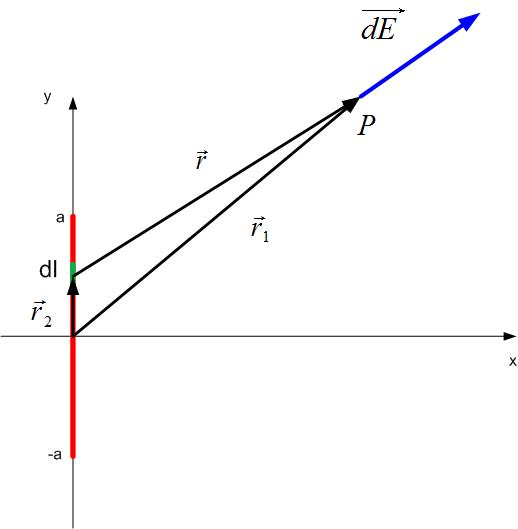
\includegraphics[scale=0.5]{../jpg/stickf.jpg}
\caption{\label{stickf} Loop of wire uniformly charged with line charge density $\rho_l$. Electric field is shown due to a very small section (arc length) of the loop $dl$.}
\end{center}
\end{figure}

\section{Potential}

\subsection{Derive Analytical Solution for the Potential  Due to a Loop of Charge }

Derive the potential due to a ring of charge, charged with a line charge density $\rho_l$. 


Potential due to a point charge is given in Equation \ref{genpotloop}. We will first find the potential due to a loop of charge. Assume that the loop of charge is charged with the line charge density $\rho_l$. The loop of charge is in X-Y plane, as shown in Figure \ref{loopanyptf}.  First we will divide the loop into small pieces. We will assume that the small  arc obtained in this way can be considered a point charge. The potential due to a point charge at a point P is labeled  in Figure \ref{loopanyptf} as $dV$.  The position of the point charge is defined by a position vector $\vec{r_2}$. The position of point P is defined with the position vector  $\vec{r_1}$. The electric scalar potential $dV$ is defined in  Equation  \ref{genpotloop}.


\begin{eqnarray}
dV=\frac{dQ}{4 \pi \epsilon_{0} {r}}  \label{genpotloop}
\end{eqnarray}


\begin{figure}[htbp]
\begin{center}
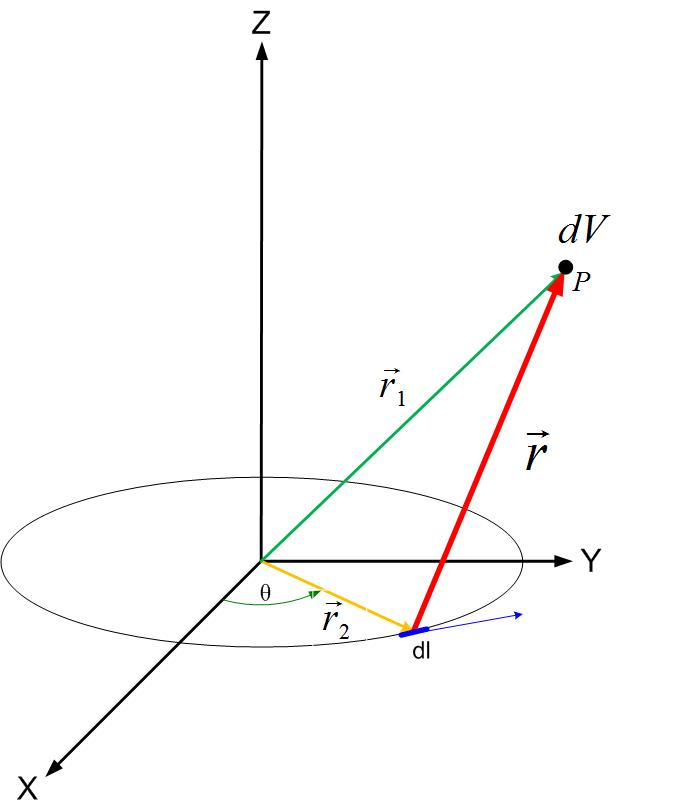
\includegraphics[scale=0.3]{../jpg/Charge_Distributionanypointpot.jpg}
%\strut\psfig{figure=chargedistribution.ps,width=3cm} \\
\end{center}
\caption{Loop of wire uniformly charged with line charge density $\rho_l$. Electric field is shown due to a very small section (arc length) of the loop $dl$.}
\label{loopanyptf}
\end{figure}

The total potential at a point P is then equal to the sum of all the potentials due to the point charges as shown in figure \ref{loopanypt1}. The equation for the total potential is given in \ref{eqtotfieldringpot}. 

\begin{eqnarray}
V=\int\limits_{all \,\, point \,\, charges} dV \label{eqtotfieldringpot}
\end{eqnarray}

\begin{figure}[htbp]
\begin{center}
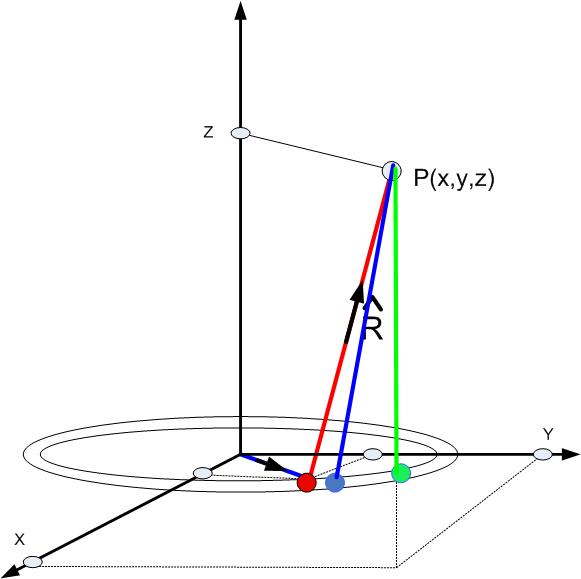
\includegraphics[scale=0.4]{../jpg/ringefieldanywheremorechargespot.jpg}
%\strut\psfig{figure=chargedistribution.ps,width=3cm} \\
\end{center}
\caption{Loop of wire uniformly charged with line charge density $\rho_l$. Electric field is shown due to several very small sections (arc length) of the loop $dl$.
Each section is modeled by a point charge $dQ$.}
\label{loopanypt1}
\end{figure}



The problem now  is to represent all the variables in the Equation \ref{genpotloop}  ( $dQ$, $dl$, $\hat{r}$ and $r$) using  appropriate coordinate system and given charge distribution.
The  total charge on the segment $dl$ is equal to $dQ=\rho_l dl$. As seen in Figure \ref{loopanyptf}, $dl$ is an arc length in the direction of theta (blue arrow next to $dl$) $dl=a\, d\theta$, where $ a$ is the radius of the loop. The vector $\vec{r_2}$ is the position vector of the arc length $dl$ and the vector $\vec{r_1}$  is the position vector of the point be  of the electric field calculation. Point P is an arbitrary point in the Cartesian coordinate system, P(x,y,z), therefore its  vector is shown in Equation \ref{eq1loopp}.  The vector $\vec{r}$ is the distance vector between the point charge (the source) and the point at which we are calculating the electric field. 



\begin{eqnarray}
\vec{r_1}=x \vec{a_x} + y \vec{a_y} +z\vec{a_z} \label{eq1loopp}
\end{eqnarray}

The vector $\vec{r_2}$ can be written in Polar Coordinates as in equation \ref{pcvecp},where $a$ is the radius of the loop. The Equation \ref{pcvecp} can be rewritten in Cartesian coordinate system as in Equation \ref{csloopvecp}.

\begin{eqnarray}
\vec{r_2}=a \, \vec{a_r} \label{pcvecp} \\
\vec{a_r}= \,cos{\theta} \, \vec{a_x}+ sin{\theta} \, \vec{a_y} \\
\vec{r_2}=a \, cos{\theta}\,  \vec{a_x}+ a \, sin{\theta} \, \vec{a_y} \label{csloopvecp}
\end{eqnarray}

The two vectors mark the beginning and the end of the distance vector $\vec{r}$. The vector  $\vec{r}$ is the sum of vectors $-\vec{r_2}$ and $\vec{r_1}$. 



\begin{eqnarray}
\vec{r}=\vec{r_1} + (-\vec{r_2})
\end{eqnarray}


Therefore the vector's $\vec{r}$  magnitude is shown in Equations \ref{vecrloop1p}.


\begin{eqnarray}
\vec{r}= (x -  a \,cos{\theta}) \vec{a_x} +(y - a \,sin{\theta}) \vec{a_y} +z \vec{a_z}
\end{eqnarray}

Vector $\vec{r}$ has the magnitude of:


\begin{eqnarray}
|\vec{r}|= \sqrt{(x - a \,cos{\theta})^2 +(y - a \,sin{\theta})^2 +z ^2}\label{vecrloop1p}
\end{eqnarray}

Replacing other variables in the Equations \ref{eq1loopp}-\ref{vecrloop1p} to the Equation \ref{genpotloop}, we get the    Equation \ref{totpot} for the potential $dV$ at a point P.

\begin{eqnarray}
dV= \frac{\rho_l \, a \, d\theta }{4 \pi \epsilon_{0} {  \sqrt{(x - a \,cos{\theta})^2 +(y - a \,sin{\theta})^2 +z ^2}  }}\label{totpot}
\end{eqnarray}



\begin{eqnarray}
V= \int\limits_0^{2 \pi}\frac{\rho_l \, a \, d\theta }{4 \pi \epsilon_{0} {  \sqrt{(x - a \,cos{\theta})^2 +(y - a \,sin{\theta})^2 +z ^2}  }}\label{totalfieldloopp2}
\end{eqnarray}








The integral in Equation \ref{totalfieldloopp2} can be integrated analytically in some special cases, however this equation can be solved numerically as shown in the next section.






\subsection{Derive Numerical solution to the Electric Field due to a Loop of Charge}



The integrals in equations \ref{totalfieldloopp2} can be represented with infinite sum using  simple numerical integration (trapezoidal rule) as shown in Equations \ref{totalfieldloop6np}.  Here we see that the continuous function of $\theta$ was replaced with the discrete values of  $\theta$.




\begin{eqnarray}
V=  \sum_{i=0}^{n}\frac{\rho_l \, a   \Delta \theta }{4 \pi \epsilon_{0} {  \sqrt{(x - a \,cos{\theta_i})^2 +(y - a \,sin{\theta_i})^2 +z ^2}  }}  \label{totalfieldloop6np}
\end{eqnarray}

Where $\Delta\theta$ represents the length of the interval that the line is divided into, $\theta_i$ represents the value of angle at a certain point, and $i$ designates different points on the loop. It should be noted here that the error due to trapezoidal rule can be improved by using more advanced numerical integration techniques.


\subsection{Matlab Code to Find the Electric Potenital due to a Loop of Charge }
 

 Plot the cross-section of the potential and the equipotential lines on the planes x=0, y=0, z=0. 
  \begin{verbatim}
clear all
%Specify the extents of x,y,z axes
rad=-1.5:0.1:1.5
 
%Make X,Y,Z matrices 
[X Y Z]=meshgrid(rad,rad,rad)
%Define constants epsilon, Q. They are obviously not physical. They are set 
%to small constants so that we get smaller numbers.
eps=1
Q=1
const=Q/(2*pi*eps)
%Set the initial potential value to zero. Initialize V.
V=0
%Here we find the potential at all X,Y,Z points defined previously from
%each of the "unit" charges on the ring. The th variable starts from 0.1
%to avoid the infinite value of V at the point r=1,theta=0. 
 
 for th=0.1:pi/20:2*pi
     t=const./ sqrt((X-cos(th)).^2 + (Y-sin(th)).^2 + (Z).^2)
V= V+t;
 end
 %Plot the volume distribution of potential at planes x=0, y=0, z=0
slice(X,Y,Z,V,[0],[0],[0])
%Keep the same figure
hold on;
%Plot contours of potential at planes x=0, y=0, z=0. See 
%more on contours in appendix.
h=contourslice(X,Y,Z,V,[0],[0],[0])
set(h,'EdgeColor','k','LineWidth',1.5)
\end{verbatim}


\subsubsection{ Plot several equipotential surfaces. }




\begin{verbatim}

clear all
%Specify the extents of x,y,z axes
rad=-1.5:0.1:1.5
 
%Make X,Y,Z matrices 
[X Y Z]=meshgrid(rad,rad,rad)
%Define constants epsilon, Q. They are obviously not physical. 
%They are set 
%to small constants so that we get smaller numbers.
eps=1
Q=1
const=Q/(2*pi*eps)
%Set the initial potential value to zero. Initialize V.
V=0
%Here we find the potential at all X,Y,Z points defined previously from
%each of the "unit" charges on the ring. The th variable starts from 0.1
%to avoid the infinite value of V at the point r=1,theta=0. 
 
 for th=0.1:pi/20:2*pi
     t=const./ sqrt((X-cos(th)).^2 + (Y-sin(th)).^2 + (Z).^2)
V= V+t;
 end
 %Plot the volume distribution of potential at planes x=0, y=0, z=0
p = patch(isosurface(X,Y,Z,V,7));
isonormals(X,Y,Z,V,p)
set(p,'FaceColor','red','EdgeColor','none');
daspect([1 1 1])
view(3); axis tight
camlight 
lighting gouraud
\end{verbatim}



Observe the equipotential surfaces. Explain why are the surfaces doughnut shaped? What is the electric field direction on the surface? Change the isosurface from 7 to 10 or some larger number. How does the isosurface look now? How does the potential of a ring of charge looks at the distances far away from the ring? What about field?







\section{Visualizing Scalar Fields in Matlab}

To visualize scalar fields in Matlab we can use the following functions: slice, contourslice, patch, isonormals, camlight and lightning. Please note that more detailed explanation about the these organization functions shown here can be found in Matlab help.

\subsection{slice}
 
Slice is a command that shows the magnitude of a scalar fields on a plane that slices the volume where the potential field is visualized. The format of this command is as shown below.

\begin{verbatim}
slice(x,y,z,v,xslice,yslice,zslice)
\end{verbatim}

Where X, Y, and Z are coordinate of points where the scaler function is calculated, V is v the scalar function at those points, and the last three vectors xslice, yslice, and zslice  are showing where will the volume will be sliced.

An example of slice command is given below. in the example below there is an additional command colormap, that's collars the volume with a specific pallette. To see more about different color maps, see Matlab help. xslice has three points at which the x-axis will be slice. They are -1.2, .8, 2. This means that the volume will be slice with a plane that is perpendicular to x-axis and it crosses the x-axis at points -1.2, .8 and 2. 
 
\begin{verbatim}
clc
clear all
[x,y,z] = meshgrid(-2:.2:2,-2:.25:2,-2:.16:2);
v = x.*exp(-x.^2-y.^2-z.^2);
xslice = [-1.2,.8,2]; yslice = 1; zslice = [-2,0];
slice(x,y,z,v,xslice,yslice,zslice)
colormap hsv
\end{verbatim}

\subsection{contourslice}

 Contourslice command will display equipotential  lines on a plane being the volume where the potential field is visualized. An example of contourslice function is shown below.

\begin{verbatim}
[x,y,z] = meshgrid(-2:.2:2,-2:.25:2,-2:.16:2);
v = x.*exp(-x.^2-y.^2-z.^2); % Create volume data
[xi,yi,zi] = sphere; % Plane to contour
contourslice(x,y,z,v,xi,yi,zi)
view(3)
\end{verbatim}

\subsection{patch}

Patch command creates a patch of color.


\subsection{isonormals}

Command isonormals creates  equipotential surfaces. 
\subsection{camlight}

\begin{verbatim}
camlight('headlight') creates a light at the camera position.camlight('right') creates a light
right and up from camera.

camlight('left') creates a light
left and up from camera.camlight with no arguments is the
same as camlight('right').

camlight(az,el) creates a light
at the specified azimuth (az) and elevation (el)
with respect to the camera position. The camera target is the center of rotation
and az and el are in degrees.

\end{verbatim}



\subsection{lighting}


\begin{verbatim}
lighting flat selects flat lighting.

lighting gouraud selects gouraud lighting.

lighting phong selects phong lighting.

lighting none turns off lighting.
\end{verbatim}








\end{document} 
